\documentclass{standalone}
\usepackage{tikz}
\usetikzlibrary{patterns, positioning}


\begin{document}
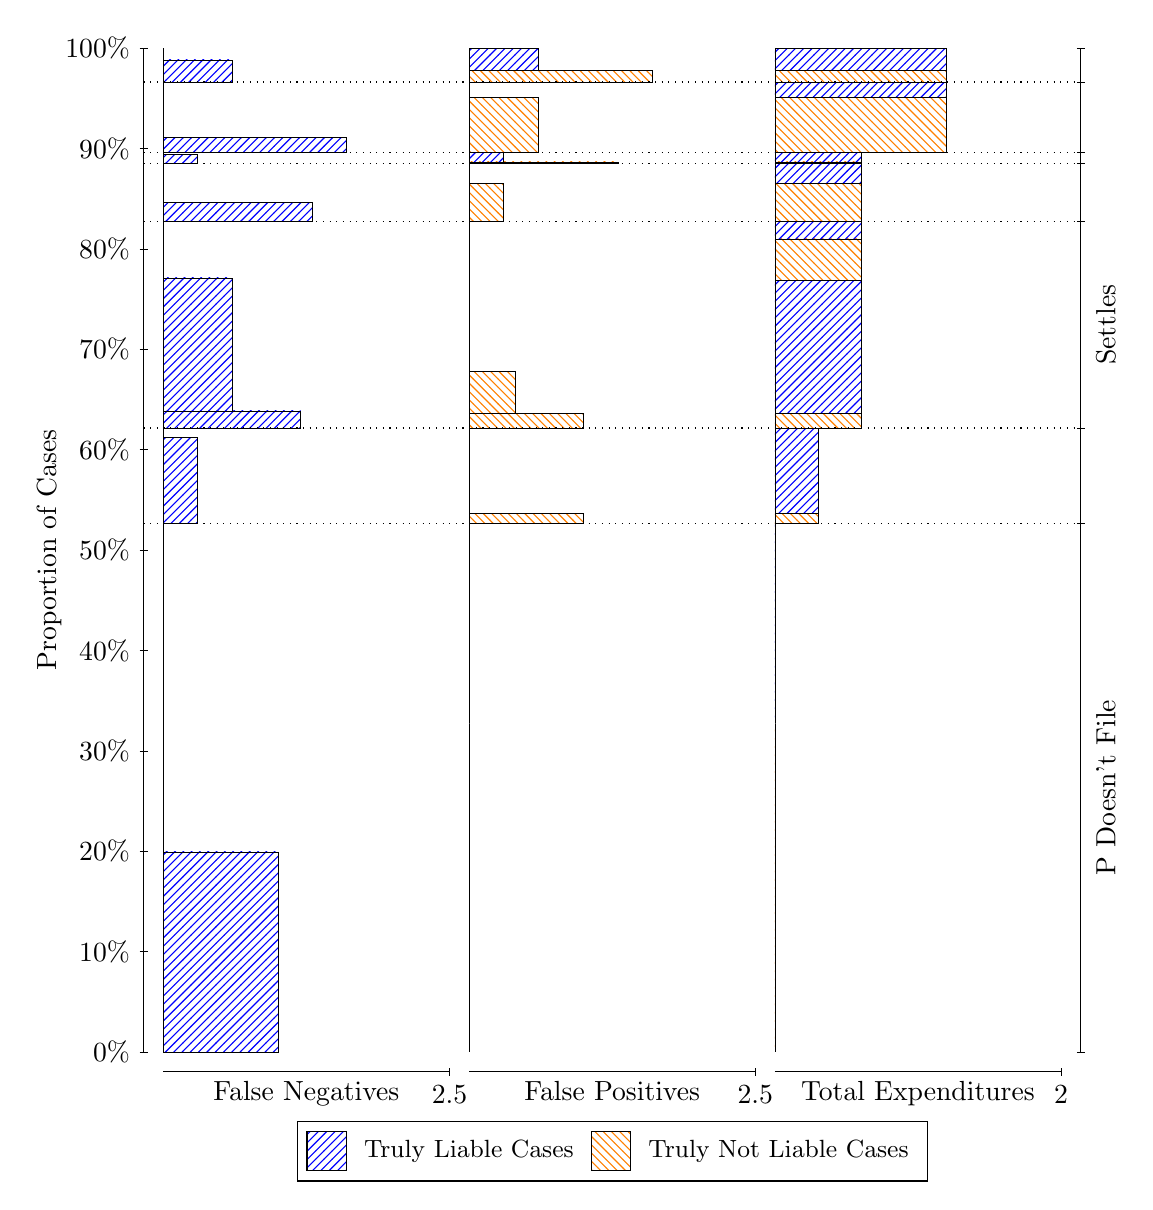
\begin{tikzpicture}
\draw[black, very thin] (1.5,1.75) -- (1.5,14.5);
\node[rotate=90, text=black, anchor=center] at (0.3, 8.125) {Proportion of Cases};
\draw[black, very thin] (1.45,1.75) -- (1.55,1.75);
\node[text=black, anchor=east] at (1.45, 1.75) {0\%};
\draw[black, very thin] (1.45,3.025) -- (1.55,3.025);
\node[text=black, anchor=east] at (1.45, 3.025) {10\%};
\draw[black, very thin] (1.45,4.3) -- (1.55,4.3);
\node[text=black, anchor=east] at (1.45, 4.3) {20\%};
\draw[black, very thin] (1.45,5.575) -- (1.55,5.575);
\node[text=black, anchor=east] at (1.45, 5.575) {30\%};
\draw[black, very thin] (1.45,6.85) -- (1.55,6.85);
\node[text=black, anchor=east] at (1.45, 6.85) {40\%};
\draw[black, very thin] (1.45,8.125) -- (1.55,8.125);
\node[text=black, anchor=east] at (1.45, 8.125) {50\%};
\draw[black, very thin] (1.45,9.4) -- (1.55,9.4);
\node[text=black, anchor=east] at (1.45, 9.4) {60\%};
\draw[black, very thin] (1.45,10.675) -- (1.55,10.675);
\node[text=black, anchor=east] at (1.45, 10.675) {70\%};
\draw[black, very thin] (1.45,11.95) -- (1.55,11.95);
\node[text=black, anchor=east] at (1.45, 11.95) {80\%};
\draw[black, very thin] (1.45,13.225) -- (1.55,13.225);
\node[text=black, anchor=east] at (1.45, 13.225) {90\%};
\draw[black, very thin] (1.45,14.5) -- (1.55,14.5);
\node[text=black, anchor=east] at (1.45, 14.5) {100\%};

\draw[black, very thin] (13.4,1.75) -- (13.4,14.5);
\draw[black, very thin] (13.35,1.75) -- (13.45,1.75);
\node[anchor=west] at (13.35, 1.75) {};
\draw[black, very thin] (13.35,8.4635) -- (13.45,8.4635);
\node[anchor=west] at (13.35, 8.4635) {};
\draw[black, very thin] (13.35,9.6738) -- (13.45,9.6738);
\node[anchor=west] at (13.35, 9.6738) {};
\draw[black, very thin] (13.35,12.296) -- (13.45,12.296);
\node[anchor=west] at (13.35, 12.296) {};
\draw[black, very thin] (13.35,13.031) -- (13.45,13.031);
\node[anchor=west] at (13.35, 13.031) {};
\draw[black, very thin] (13.35,13.173) -- (13.45,13.173);
\node[anchor=west] at (13.35, 13.173) {};
\draw[black, very thin] (13.35,14.068) -- (13.45,14.068);
\node[anchor=west] at (13.35, 14.068) {};
\draw[black, very thin] (13.35,14.5) -- (13.45,14.5);
\node[anchor=west] at (13.35, 14.5) {};

\draw[black, very thin, pattern color=blue, pattern=north east lines] (1.75,1.75) rectangle (3.2033,4.2911);
\draw[black, very thin, pattern color=orange, pattern=north west lines] (1.75,4.2911) rectangle (1.75,8.4635);
\draw[black, very thin, pattern color=blue, pattern=north east lines] (1.75,8.4635) rectangle (2.186,9.5519);
\draw[black, very thin, pattern color=orange, pattern=north west lines] (1.75,9.5519) rectangle (1.75,9.6738);
\draw[black, very thin, pattern color=blue, pattern=north east lines] (1.75,9.6738) rectangle (3.494,9.8927);
\draw[black, very thin, pattern color=blue, pattern=north east lines] (1.75,9.8927) rectangle (2.622,11.581);
\draw[black, very thin, pattern color=orange, pattern=north west lines] (1.75,11.581) rectangle (1.75,12.296);
\draw[black, very thin, pattern color=blue, pattern=north east lines] (1.75,12.296) rectangle (3.6393,12.543);
\draw[black, very thin, pattern color=orange, pattern=north west lines] (1.75,12.543) rectangle (1.75,13.031);
\draw[black, very thin, pattern color=blue, pattern=north east lines] (1.75,13.031) rectangle (2.186,13.149);
\draw[black, very thin, pattern color=orange, pattern=north west lines] (1.75,13.149) rectangle (1.75,13.173);
\draw[black, very thin, pattern color=blue, pattern=north east lines] (1.75,13.173) rectangle (4.0753,13.366);
\draw[black, very thin, pattern color=orange, pattern=north west lines] (1.75,13.366) rectangle (1.75,14.068);
\draw[black, very thin, pattern color=blue, pattern=north east lines] (1.75,14.068) rectangle (2.622,14.348);
\draw[black, very thin, pattern color=orange, pattern=north west lines] (1.75,14.348) rectangle (1.75,14.5);
\draw[black, very thin, pattern color=orange, pattern=north west lines] (5.6333,1.75) rectangle (5.6333,5.9224);
\draw[black, very thin, pattern color=blue, pattern=north east lines] (5.6333,5.9224) rectangle (5.6333,8.4635);
\draw[black, very thin, pattern color=orange, pattern=north west lines] (5.6333,8.4635) rectangle (7.0867,8.5854);
\draw[black, very thin, pattern color=blue, pattern=north east lines] (5.6333,8.5854) rectangle (5.6333,9.6738);
\draw[black, very thin, pattern color=orange, pattern=north west lines] (5.6333,9.6738) rectangle (7.0867,9.8628);
\draw[black, very thin, pattern color=orange, pattern=north west lines] (5.6333,9.8628) rectangle (6.2147,10.389);
\draw[black, very thin, pattern color=blue, pattern=north east lines] (5.6333,10.389) rectangle (5.6333,12.296);
\draw[black, very thin, pattern color=orange, pattern=north west lines] (5.6333,12.296) rectangle (6.0693,12.784);
\draw[black, very thin, pattern color=blue, pattern=north east lines] (5.6333,12.784) rectangle (5.6333,13.031);
\draw[black, very thin, pattern color=orange, pattern=north west lines] (5.6333,13.031) rectangle (7.5227,13.055);
\draw[black, very thin, pattern color=blue, pattern=north east lines] (5.6333,13.055) rectangle (6.0693,13.173);
\draw[black, very thin, pattern color=orange, pattern=north west lines] (5.6333,13.173) rectangle (6.5053,13.874);
\draw[black, very thin, pattern color=blue, pattern=north east lines] (5.6333,13.874) rectangle (5.6333,14.068);
\draw[black, very thin, pattern color=orange, pattern=north west lines] (5.6333,14.068) rectangle (7.9587,14.22);
\draw[black, very thin, pattern color=blue, pattern=north east lines] (5.6333,14.22) rectangle (6.5053,14.5);
\draw[black, very thin, pattern color=orange, pattern=north west lines] (9.5167,1.75) rectangle (9.5167,5.9224);
\draw[black, very thin, pattern color=blue, pattern=north east lines] (9.5167,5.9224) rectangle (9.5167,8.4635);
\draw[black, very thin, pattern color=orange, pattern=north west lines] (9.5167,8.4635) rectangle (10.062,8.5854);
\draw[black, very thin, pattern color=blue, pattern=north east lines] (9.5167,8.5854) rectangle (10.062,9.6738);
\draw[black, very thin, pattern color=orange, pattern=north west lines] (9.5167,9.6738) rectangle (10.607,9.8628);
\draw[black, very thin, pattern color=blue, pattern=north east lines] (9.5167,9.8628) rectangle (10.607,11.551);
\draw[black, very thin, pattern color=orange, pattern=north west lines] (9.5167,11.551) rectangle (10.607,12.077);
\draw[black, very thin, pattern color=blue, pattern=north east lines] (9.5167,12.077) rectangle (10.607,12.296);
\draw[black, very thin, pattern color=orange, pattern=north west lines] (9.5167,12.296) rectangle (10.607,12.784);
\draw[black, very thin, pattern color=blue, pattern=north east lines] (9.5167,12.784) rectangle (10.607,13.031);
\draw[black, very thin, pattern color=orange, pattern=north west lines] (9.5167,13.031) rectangle (10.607,13.055);
\draw[black, very thin, pattern color=blue, pattern=north east lines] (9.5167,13.055) rectangle (10.607,13.173);
\draw[black, very thin, pattern color=orange, pattern=north west lines] (9.5167,13.173) rectangle (11.697,13.874);
\draw[black, very thin, pattern color=blue, pattern=north east lines] (9.5167,13.874) rectangle (11.697,14.068);
\draw[black, very thin, pattern color=orange, pattern=north west lines] (9.5167,14.068) rectangle (11.697,14.22);
\draw[black, very thin, pattern color=blue, pattern=north east lines] (9.5167,14.22) rectangle (11.697,14.5);
\draw[black, dotted] (1.5,8.4635) -- (13.4,8.4635);
\draw[black, dotted] (1.5,9.6738) -- (13.4,9.6738);
\draw[black, dotted] (1.5,12.296) -- (13.4,12.296);
\draw[black, dotted] (1.5,13.031) -- (13.4,13.031);
\draw[black, dotted] (1.5,13.173) -- (13.4,13.173);
\draw[black, dotted] (1.5,14.068) -- (13.4,14.068);
\draw[black, very thin] (1.75,1.5) -- (5.3833,1.5);
\node[text=black, anchor=north] at (3.5667, 1.5) {False Negatives};
\draw[black, very thin] (5.3833,1.45) -- (5.3833,1.55);
\node[text=black, anchor=north] at (5.3833, 1.45) {2.5};

\draw[black, very thin] (5.6333,1.5) -- (9.2667,1.5);
\node[text=black, anchor=north] at (7.45, 1.5) {False Positives};
\draw[black, very thin] (9.2667,1.45) -- (9.2667,1.55);
\node[text=black, anchor=north] at (9.2667, 1.45) {2.5};

\draw[black, very thin] (9.5167,1.5) -- (13.15,1.5);
\node[text=black, anchor=north] at (11.333, 1.5) {Total Expenditures};
\draw[black, very thin] (13.15,1.45) -- (13.15,1.55);
\node[text=black, anchor=north] at (13.15, 1.45) {2};

\node[text=black, centered, rotate=90] at (13.72, 5.1067) {P Doesn't File};

\node[text=black, centered, rotate=90] at (13.72, 10.985) {Settles};





\draw (7.449999999999999,1.5) node[draw=none] (baseCoordinate) {};
\begin{scope}[align=center]
        \matrix[scale=0.5, draw=black, below=0.5cm of baseCoordinate, nodes={draw}, column sep=0.1cm]{
            \node[rectangle, draw, minimum width=0.5cm, minimum height=0.5cm, pattern color=blue, pattern=north east lines] {}; &
            \node[draw=none, font=\small, text=black] (B) {Truly Liable Cases}; &
            \node[rectangle, draw, minimum width=0.5cm, minimum height=0.5cm, pattern color=orange, pattern=north west lines] {}; &
            \node[draw=none, font=\small, text=black] (B) {Truly Not Liable Cases}; \\
            };
\end{scope}

\end{tikzpicture}
\end{document}